\documentclass[11pt,a4paper]{article}
\usepackage[margin=2.2cm]{geometry}
\usepackage{graphicx,booktabs,amsmath,amssymb,array,xcolor,enumitem,float,caption,catchfile}
\usepackage[hidelinks]{hyperref}
\graphicspath{{../figures/}}
\setlist{nosep,leftmargin=1.4em}
% tables generated by code/experiments.py (loaded here because \input cannot start a table row)
\CatchFileDef\TabNodes{../results/table_nodes.tex}{}
\CatchFileDef\TabCases{../results/table_cases.tex}{}
\CatchFileDef\TabArena{../results/table_arena.tex}{}
\CatchFileDef\TabGamesB{../results/table_games_b.tex}{}
\newcommand{\DMAX}{4}
\newcommand{\WoneMM}{3,202}
\newcommand{\WoneAB}{419}
\newcommand{\WtwoMM}{1,923}
\newcommand{\WtwoAB}{112}
\newcommand{\EoneABfour}{34,023}
\newcommand{\ItalWorst}{403,780}
\newcommand{\ItalMVV}{7,372}
\newcommand{\MidMM}{4,701,529}
\newcommand{\MidAB}{34,023}
\newcommand{\AvgMM}{1,217,272}
\newcommand{\AvgAB}{9,370}
\newcommand{\AgreePos}{636}
\newcommand{\AgreeMove}{98.7}
\newcommand{\AgreeValue}{100.0}

\title{\textbf{Multi-Agent Chess Arena}\\[4pt]
\large A Minimax Agent vs.\ an Alpha-Beta Pruning Agent with Heuristic Evaluation\\[2pt]
\normalsize 23CSE401 -- Fundamentals of Artificial Intelligence: Case Study}
\author{Name: Nikhil Sanjay \qquad Roll No.: BL.EN.U4CSE23239}
\date{}
\begin{document}
\maketitle

\begin{abstract}
We build a chess arena in which two game-playing agents compete: a depth-limited
\textbf{Minimax} agent and an \textbf{Alpha-Beta} agent. Both use the same heuristic evaluation
(material plus piece-square tables), so every difference between them comes from the search
technique. On five test positions at depths 1--4, alpha-beta returned exactly the minimax value in every run
while visiting far fewer positions. At depth 4 from the starting position it searched 3,109 nodes against
206,604 for minimax. Two working cases (a mate and a fork) and three edge cases (the horizon effect, a
stalemate trap and bad move ordering) show how the agents behave in normal and difficult positions. In a
24-game arena, equal-depth agents play at the same strength, but when alpha-beta spends its savings on one extra ply of
search, at less than twice minimax's node budget, it scores 8.5--3.5.
\end{abstract}

%=====================================================================
\section{Problem Domain and Statement}
\textbf{Domain.} Chess: a two-player, turn-based board game on an $8\times8$ board. White and Black
each start with 16 pieces and alternate moves. A player wins by checkmating the opponent's king. A game
can also end in a draw (stalemate, threefold repetition, insufficient material, 50-move rule).

\textbf{Agents.} Two software agents play each other in an \emph{arena} (a game loop that
asks the side to move for a move, applies it and checks for the end of the game):
\begin{itemize}
\item \textbf{Minimax agent (MM):} looks ahead $d$ plies and considers \emph{every} sequence of legal
moves. It scores the positions at depth $d$ with a heuristic and backs the values up the tree.
\item \textbf{Alpha-Beta agent (AB):} the same look-ahead and the same heuristic, but it
\emph{prunes} branches that provably cannot change the decision. It also orders moves (captures first) so that
pruning happens early.
\end{itemize}

\textbf{Goals.} Each agent tries to maximise its own game outcome (win $>$ draw $>$ loss).
Chess is zero-sum, so one agent's gain is exactly the other's loss.

\textbf{Interaction.} The agents share one board and move alternately. Every move changes the
options of the opponent, and each agent has to predict the other's reply. This is what makes the problem
multi-agent and adversarial.

\textbf{Problem statement.} Given a chess position, choose a move that is best for the side to move,
assuming the opponent also plays its best replies, within a limited amount of computation.
Then measure (i) whether the two search techniques choose equally good moves, (ii) how much
computation each needs and (iii) how this translates into results when the agents play each other.

%=====================================================================
\section{PEAS Description}
\begin{center}
\begin{tabular}{>{\bfseries}p{3.1cm}p{12.6cm}}
\toprule
Performance measure & Game result (win = 1, draw = $\tfrac12$, loss = 0) over many games; material balance;
quality of each chosen move (its minimax value); computational cost per move (nodes searched, time). \\
Environment & The $8\times8$ board with its pieces, the opponent agent, and the rules of chess
(legal moves, check, checkmate, stalemate, repetition, promotion, castling, en passant). Rules are provided by the
\texttt{python-chess} library. \\
Actuators & Selecting and playing one legal move on the agent's turn (a piece move, capture,
castling, en-passant capture or promotion). \\
Sensors & The complete board state (FEN): piece placement, side to move, castling rights,
en-passant square and move counters; the list of legal moves; whether the position is check, checkmate or a draw. \\
\bottomrule
\end{tabular}
\end{center}

%=====================================================================
\section{Environment Properties}
\begin{center}
\begin{tabular}{>{\bfseries}p{2.9cm}p{2.7cm}p{9.5cm}}
\toprule
Property & Value & Justification \\
\midrule
Observability & Fully observable & Both agents see the whole board and every piece. Nothing is hidden (unlike poker). \\
Determinism & Deterministic & A move always has exactly the stated effect; there is no chance element.
The only uncertainty is the opponent's choice, which is handled by adversarial search, not probabilities. \\
Episodic / sequential & Sequential & Every move affects all later positions. A pawn grabbed now can lose the queen
two moves later (case E1). \\
Static / dynamic & Static & The board does not change while an agent is thinking. (With a chess clock it would be
\emph{semi-dynamic}: the position stays fixed but the remaining time shrinks.) \\
Discrete / continuous & Discrete & 64 squares, a finite set of legal moves, and discrete turns. \\
Single / multi-agent & Multi-agent & Two agents whose objectives are exactly opposed (competitive, zero-sum). \\
Known / unknown & Known & The rules, i.e.\ the transition model, are fully known to both agents. \\
\bottomrule
\end{tabular}
\end{center}

%=====================================================================
\section{Type of Agent}
Both players are \textbf{utility-based, model-based agents with adversarial look-ahead}:
\begin{itemize}
\item \emph{Model-based}: the agent uses the rules of chess (the transition model $\textsc{Result}(s,a)$) to
simulate moves internally before playing one.
\item \emph{Utility-based}: a goal test (``is it checkmate?'') is almost never reachable within the search horizon, so
the agent needs a \emph{utility estimate} of non-terminal positions. That estimate is the heuristic evaluation
function of Section~\ref{sec:eval}. The agent picks the move with the best backed-up utility.
\end{itemize}
A \emph{simple reflex} agent (e.g.\ ``capture the most valuable piece'') is not enough. In case E2 it
captures a knight and stalemates a completely won position. A \emph{goal-based} agent without a utility
estimate cannot rank moves when no mate is in sight.

\textbf{Cooperative or competitive?} The agents are \textbf{purely competitive}. Chess is a
two-player \emph{zero-sum} game: $U_{\text{White}}=-U_{\text{Black}}$. There is no joint objective and
no communication. Each agent therefore models the other as an adversary that always chooses the reply worst for
it, which is exactly the assumption behind minimax: White is MAX, Black is MIN.
Within each agent the search is a solo computation, and the two agents never cooperate.

%=====================================================================
\section{Heuristic Evaluation Function}\label{sec:eval}
Both agents use one evaluation, from White's point of view in centipawns (100 = one pawn):
\[
\mathrm{eval}(s)=\sum_{p\,\in\,\text{White}}\big(V(p)+\mathrm{PST}_p(\text{sq})\big)\;-\;\sum_{p\,\in\,\text{Black}}\big(V(p)+\mathrm{PST}_p(\text{sq})\big)
\]
with piece values $V$ = P~100, N~320, B~330, R~500, Q~900, and Michniewski's piece-square tables
$\mathrm{PST}$. These reward centralised knights, advanced pawns and a castled king, and penalise knights on the rim.
Terminal positions are scored exactly: checkmate $=\pm(100000-\text{ply})$, so a faster mate is preferred,
while stalemate and insufficient material score 0. The evaluation is cheap ($O(\text{pieces})$) but ignores king
safety, mobility and threats. Section~\ref{sec:cases} shows the consequences.

%=====================================================================
\section{Searching Technique}
\subsection{Formulation as a search problem}
\begin{itemize}
\item \textbf{State:} a chess position (board, side to move, castling/en-passant rights).
\item \textbf{Initial state:} the current position. \quad \textbf{Players:} MAX = White, MIN = Black.
\item \textbf{Actions:} the legal moves (on average $b\approx35$ in the middlegame, 20 at the start).
\item \textbf{Terminal test:} checkmate, stalemate, insufficient material.
\item \textbf{Utility / cut-off:} at depth $d$ the heuristic replaces the true game value.
\end{itemize}
The state space of chess has about $10^{43}$--$10^{47}$ positions and the game tree about $10^{120}$ nodes
(Shannon), so the search must be depth-limited.

\subsection{Minimax}
\[
\textsc{MM}(s,d)=\begin{cases}
\mathrm{eval}(s) & d=0 \text{ or terminal}\\
\max_a \textsc{MM}(\textsc{Result}(s,a),d-1) & \text{White to move}\\
\min_a \textsc{MM}(\textsc{Result}(s,a),d-1) & \text{Black to move}
\end{cases}
\]
The recursion is a depth-first traversal of the whole tree to depth $d$. The agent plays the root move with the best
backed-up value.

\subsection{Alpha-beta pruning}
Alpha-beta computes the same $\textsc{MM}(s,d)$ but carries two bounds: $\alpha$, the best value MAX is already
guaranteed on the current path, and $\beta$, the best value MIN is already guaranteed. At a MIN node, as soon
as one reply gives a value $\le\alpha$, MAX will never enter this node, because it already has something better. The
remaining replies are therefore skipped (a \emph{cut-off}). The same holds symmetrically at MAX nodes.
Pruning never changes the result. It only avoids work, and our experiments \texttt{assert} this on every run.
The amount of pruning depends on the order in which moves are tried. Our AB agent sorts moves by
\textbf{MVV-LVA} (captures of the Most Valuable Victim by the Least Valuable Attacker first), then promotions and checks.

\subsection{State space, search tree and sequence of explored states}
To make the tree readable, Figure~\ref{fig:tree} uses a small king-and-pawn endgame
(\texttt{8/8/8/4k3/8/8/4P3/4K3 w}) at depth 2, and both searches use the same (generator) move order.
White has 6 moves and Black 6--8 replies. The sequence explored by alpha-beta is:
\begin{enumerate}
\item \textbf{Kf2}: all 8 replies searched; the minimum is 100, so $\alpha=100$.
\item \textbf{Kd2}: the first reply Kf6 already scores $100\le\alpha$. MIN can hold White to 100 here, so Kd2
cannot beat Kf2, and the other \textbf{7 replies are pruned}.
\item \textbf{Kf1}: every reply is $\ge110>\alpha$, so all are searched; the minimum is 110 and $\alpha$ becomes 110.
\item \textbf{Kd1}: first reply 100 $\le\alpha$, so \textbf{7 replies are pruned}.
\item \textbf{e3}: minimum 120, so $\alpha=120$ (the new best move).
\item \textbf{e4}: the reply ...Kxe4 wins the pawn (value 0 $\le\alpha$), so the last reply is pruned.
\end{enumerate}
Minimax evaluates all 51 positions and alpha-beta 36. Both pick \textbf{e3} with value 120.

\begin{figure}[H]\centering
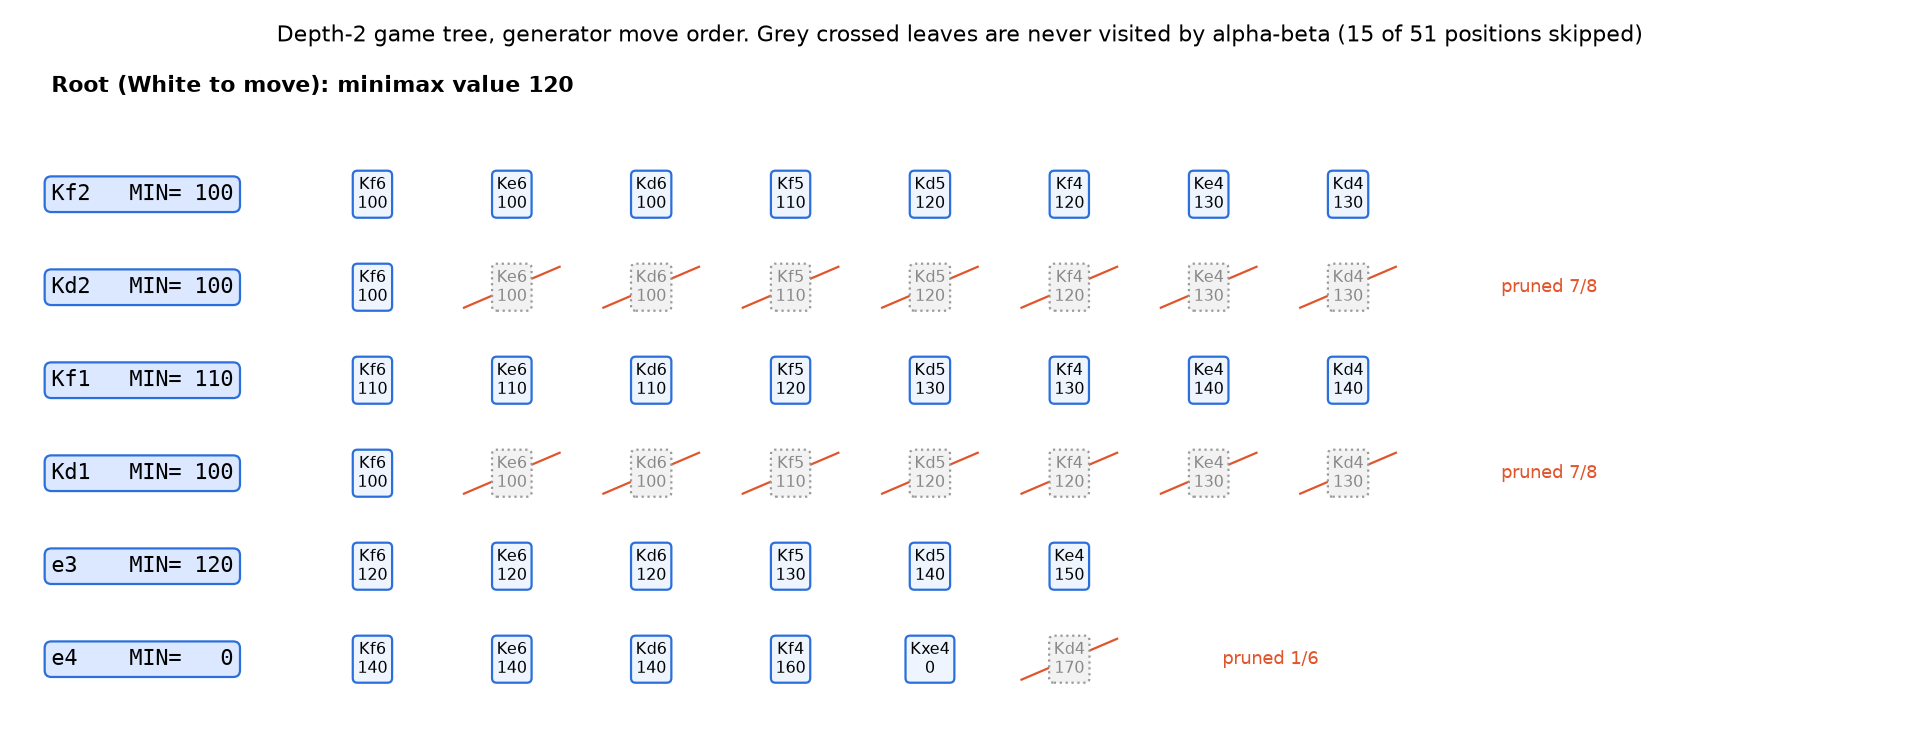
\includegraphics[width=\linewidth]{search_tree.png}
\caption{Depth-2 game tree. Blue boxes are MIN nodes (after White's move) with their backed-up values. Leaves
show Black's reply and the heuristic value. Grey, crossed leaves are skipped by alpha-beta.}
\label{fig:tree}
\end{figure}

%=====================================================================
\section{Working Cases and Edge Cases}\label{sec:cases}
Table~\ref{tab:cases} lists the move, value and cost of both agents at depths 1--4 in every case. Values
are from White's point of view; ``mate (+)'' means a forced mate for White was found.

\begin{table}[H]\centering\small
\caption{Case results (depth-4 minimax on E1 is omitted: about 4 million nodes, and alpha-beta gives the same value).}
\label{tab:cases}
\begin{tabular}{llcllrr}
\toprule
Case & Agent & Depth & Move & Value & Nodes & Time (ms) \\
\midrule
\TabCases
\bottomrule
\end{tabular}
\end{table}

\begin{figure}[H]\centering
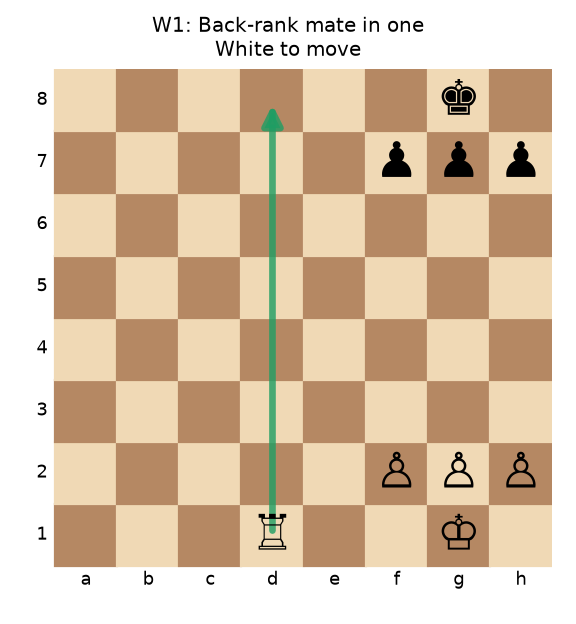
\includegraphics[width=0.24\linewidth]{case_W1.png}\hfill
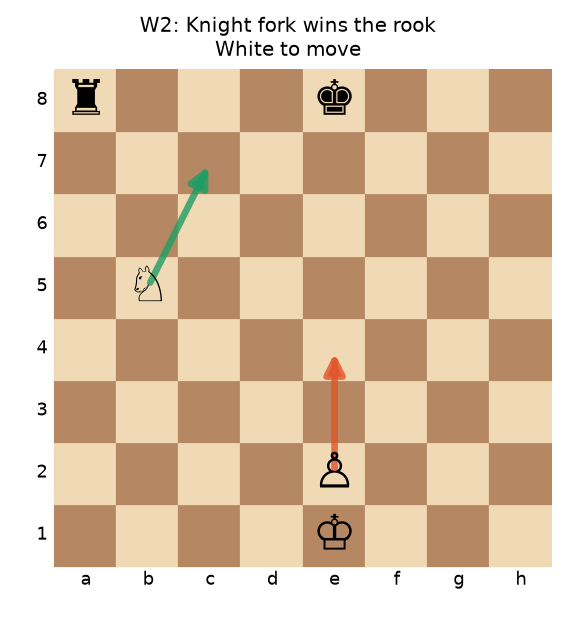
\includegraphics[width=0.24\linewidth]{case_W2.png}\hfill
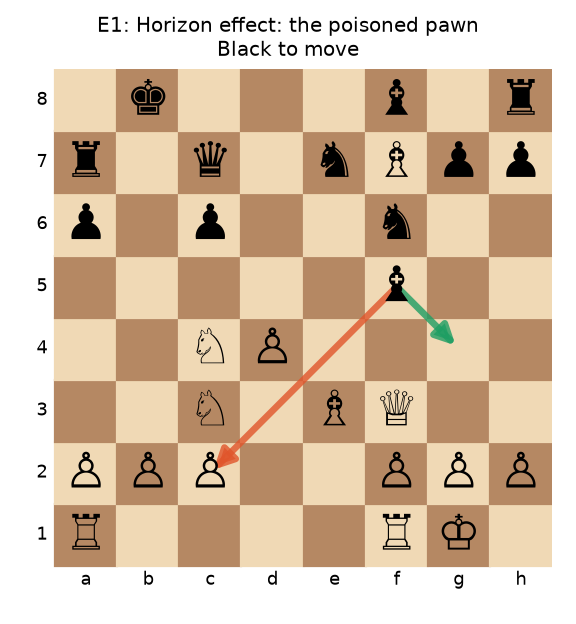
\includegraphics[width=0.24\linewidth]{case_E1.png}\hfill
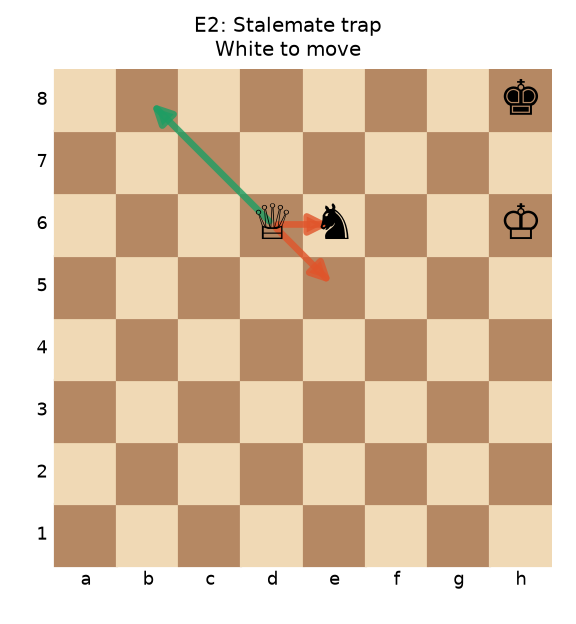
\includegraphics[width=0.24\linewidth]{case_E2.png}
\caption{Case positions. Green = move chosen at the deepest search; orange = the tempting wrong move
(shallow search or greedy capture).}
\end{figure}

\subsection*{Working case W1 -- Back-rank mate in one}
White: Kg1, Rd1, pawns f2 g2 h2; Black: Kg8, pawns f7 g7 h7. \textbf{Rd8\#} mates because Black's own
pawns block the king. Both agents find it at every depth $\ge1$, since the terminal test scores the
position after Rd8 as a mate. The mate score $100000-\text{ply}$ makes a mate-in-1 beat any material
gain. Minimax needs \WoneMM\ nodes at depth 3 against \WoneAB\ for alpha-beta. Once the mating move is searched first
(it gives check, so it is ordered early), all alternatives are cut off quickly.

\subsection*{Working case W2 -- Knight fork}
White: Ke1, Nb5, pawn e2; Black: Ke8, Ra8. \textbf{Nc7+} checks the king and attacks the rook. After the forced
king move, Nxa8 wins the rook. At depths 1--2 the agents cannot see the capture (it is ply 3) and play
the quiet pawn move e4 with a negative value, because Black is up the exchange. From depth 3 both agents play Nc7+ with
a positive value. This is the normal case: the tactic is within the horizon, both searches agree, and alpha-beta
needs \WtwoAB\ nodes against \WtwoMM.

\subsection*{Edge case E1 -- The horizon effect (from a real arena game)}
This position occurred in one of our agent games (Black to move). At depths 1 and 2 Black plays
\textbf{...Bxc2}, winning a pawn. The refutation is \textbf{Bf4!}, which pins the black queen on c7 to the
king on b8. The queen is lost \emph{on the following moves}, beyond a 2-ply horizon. The shallow search thinks
it has won a pawn (value 615 from White's view, i.e.\ better for Black than the alternatives), while the depth-4 search
evaluates ...Bxc2 at +850 and prefers \textbf{...Bg4} (+390). This is the classic \emph{horizon effect}: a
depth-limited agent cannot see a consequence one ply past its cut-off, and alpha-beta suffers exactly as much as
minimax at the same depth. The fix is to search deeper, which alpha-beta makes affordable (depth 4 here takes
alpha-beta \EoneABfour\ nodes, fewer than minimax needs at depth 3), or to add a \emph{quiescence search} that keeps
searching captures past the cut-off.

The table also shows an \emph{odd/even effect}. At odd depths Black moves last and faces no reply, so values
swing in Black's favour ($-165$ at depth 3 vs.\ $+390$ at depth 4 for the same best move).

\subsection*{Edge case E2 -- Stalemate trap}
White: Kh6, Qd6; Black: Kh8, Ne6. \textbf{Qxe6} wins a knight, and a greedy agent that counts material plays it,
but it leaves Black with no legal move and not in check: \emph{stalemate}, a draw. Our agents score stalemate as 0, so
at depth 1 Qxe6 is worth 0 and they choose another move. From depth 3 they find a \emph{forced mate}
beginning with \textbf{Qb8+}. Note the tie at depth 1: minimax plays Kh5 and alpha-beta plays Qe5+, both valued 520. With
equal values the move depends only on the order in which moves are examined. This is why equal-depth games between the
two agents can differ (Section~\ref{sec:arena}).

\subsection*{Edge case E3 -- Worst-case move ordering}
Alpha-beta's savings are not guaranteed. Table~\ref{tab:nodes} runs it with three orderings. With MVV-LVA,
good moves come first and refutations are found immediately. With \emph{reversed} MVV-LVA ordering (quiet, bad moves
first) cut-offs come late: in the Italian opening at depth \DMAX, alpha-beta then needs \ItalWorst\ nodes instead
of \ItalMVV. The value returned is identical in all three cases. Only the effort changes, which is the
practical meaning of the $O(b^{d/2})$ best case vs.\ $O(b^d)$ worst case.

%=====================================================================
\section{Complexity Analysis}
Let $b$ be the branching factor (legal moves per position) and $d$ the search depth in plies.
\begin{itemize}
\item \textbf{Minimax:} visits every node of the tree, so time $O(b^d)$. It is depth-first, so memory is
$O(b\,d)$ (the current path plus the move list at each level).
\item \textbf{Alpha-beta:} same memory $O(b\,d)$. Time depends on the ordering. In the worst case
nothing is pruned: $O(b^d)$. With perfect ordering Knuth and Moore showed it examines
$b^{\lceil d/2\rceil}+b^{\lfloor d/2\rfloor}-1$ leaves, i.e.\ $O(b^{d/2})$. The effective branching factor
drops from $b$ to $\sqrt b$, so \emph{in the same time alpha-beta can search about twice as deep}.
\item \textbf{In chess:} $b\approx20$ at the start and $\approx35$ in the middlegame. At $d=4$, minimax faces
$35^4\approx1.5$ million leaves while the alpha-beta minimum is $2\cdot35^2\approx2{,}450$.
\end{itemize}

\begin{figure}[H]\centering
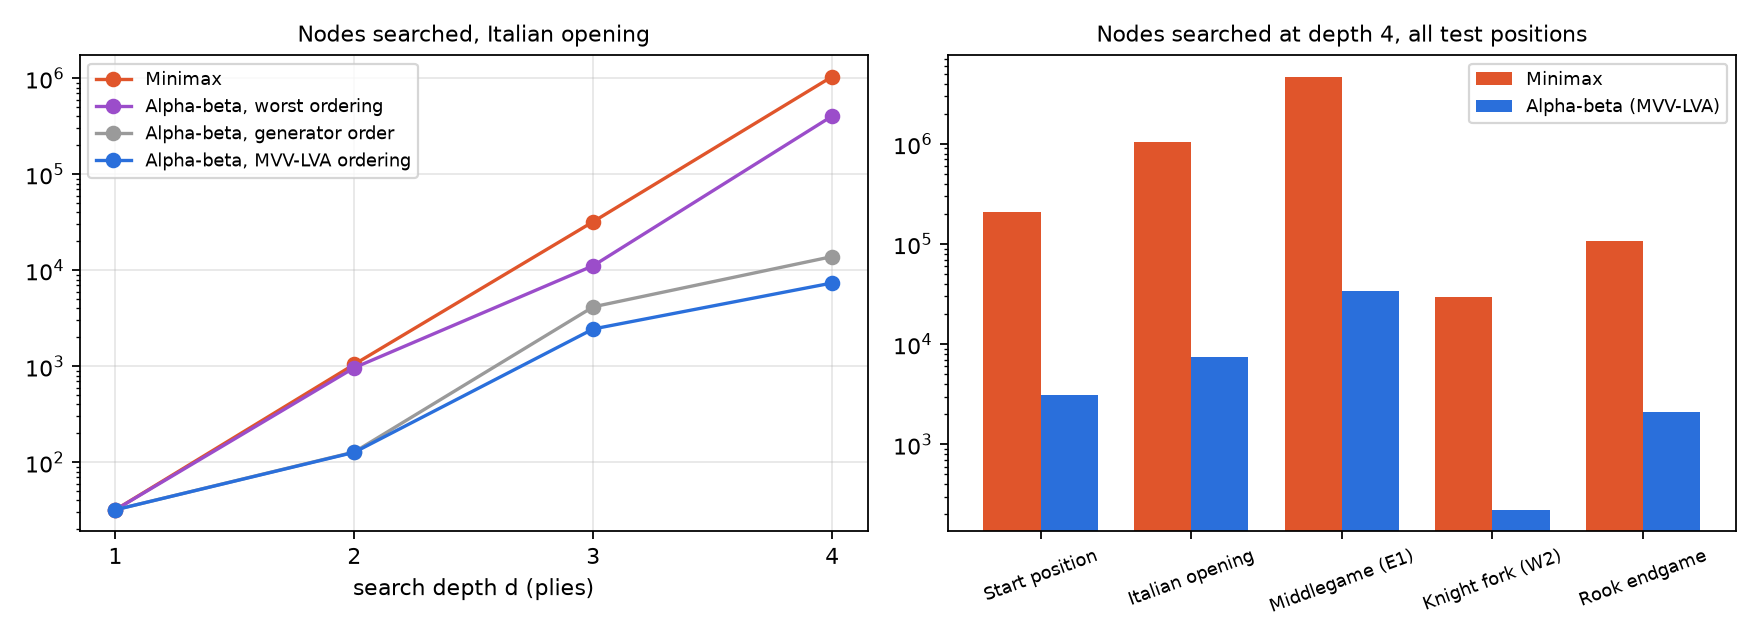
\includegraphics[width=\linewidth]{nodes_vs_depth.png}
\caption{Left: nodes searched as depth grows (log scale, Italian opening). Right: all test positions at depth \DMAX.}
\label{fig:nodes}
\end{figure}

\begin{table}[H]\centering\small
\caption{Nodes searched (root included). Worst/None/MVV = alpha-beta with reversed, generator and MVV-LVA
ordering; ``Saved'' compares MVV alpha-beta with minimax. Every row returned the same value for all four searches.}
\label{tab:nodes}
\begin{tabular}{lcllrrrrr}
\toprule
Position & $d$ & Move & Value & Minimax & AB worst & AB none & AB MVV & Saved \\
\midrule
\TabNodes
\bottomrule
\end{tabular}
\end{table}

\textbf{Relating the measurements to theory.} From the start position ($b=20$), minimax grows by a factor
of about 20--22 per ply (421 $\rightarrow$ 9,323 $\rightarrow$ 206,604), which is exactly $b$. Alpha-beta
grows by a factor of about 4--10 per ply (84 $\rightarrow$ 777 $\rightarrow$ 3,109), close to $\sqrt{b}\approx4.5$
at even steps. That is the $O(b^{d/2})$ behaviour. Its depth-4 count is 3,109, compared with a theoretical minimum of
$20^2+20^2-1=799$ leaves, so our simple ordering is good but not perfect. The middlegame position ($b=44$)
shows the gap most clearly: \MidMM\ vs.\ \MidAB\ nodes at depth \DMAX.

%=====================================================================
\section{Arena: the Agents Playing Each Other}\label{sec:arena}
Each match uses 6 openings (Italian, Sicilian, Queen's Gambit, French, English, Caro-Kann). Each opening is played twice
with the colours swapped, 12 games in total. A game is capped at 100 plies; unfinished games are adjudicated as a win
if one side leads by $\ge300$ centipawns and as a draw otherwise.

\begin{table}[H]\centering\small
\caption{Arena summary. Score = points for Minimax -- points for Alpha-beta (win 1, draw $\frac12$). Nodes and milliseconds are averages per move.}
\begin{tabular}{lcrrrrr}
\toprule
Match & Games & MM -- AB & MM nodes & AB nodes & MM ms & AB ms \\
\midrule
\TabArena
\bottomrule
\end{tabular}
\end{table}

\begin{figure}[H]\centering
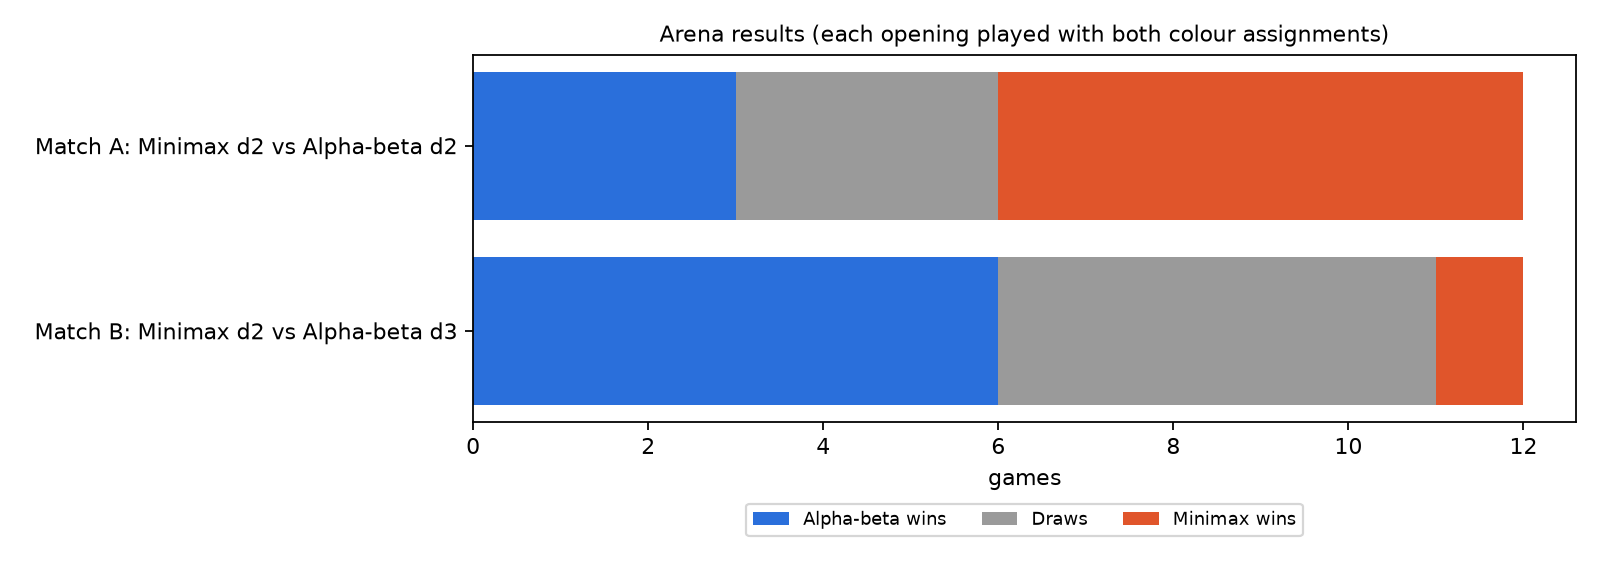
\includegraphics[width=0.85\linewidth]{arena.png}
\end{figure}

\textbf{Match A -- equal depth (both depth 2).} Minimax scored 7.5--4.5. This does \emph{not} mean minimax plays
better. We replayed all \AgreePos\ positions from these games and asked both agents for their move. The chosen moves had
the \textbf{same minimax value in \AgreeValue\% of positions}, and the agents chose the identical move in \AgreeMove\%. The few
differences are tie-breaks between equally valued moves (as in E2 at depth 1), caused by alpha-beta's different move
order. Once one tie is broken differently the two games diverge, and at depth 2 the play is weak enough (many games end
in checkmate after blunders) that such divergences decide games. With deterministic agents and 12 games the score is
essentially noise. The important column is the cost: alpha-beta needed about $8\times$ fewer nodes per move for the
same decisions.

\textbf{Match B -- alpha-beta spends its savings on depth (depth 3 vs.\ depth 2).} A depth-3 minimax would need
roughly 9--93 thousand nodes per move (Table~\ref{tab:nodes}), while the depth-3 alpha-beta agent needed about 2,200, less than twice what
minimax spends at depth 2. With this extra ply the alpha-beta agent won 6 games, drew 5 and lost 1 (score 8.5--3.5).
It sees the opponent's reply to its reply, so it avoids the one-move traps that decide games at depth 2. The draws
are threefold repetitions: deterministic agents with a shallow horizon tend to shuffle pieces back and forth once no
tactic is visible, which is another face of the horizon effect.

\begin{table}[H]\centering\small
\caption{All games of Match B (MM = minimax, AB = alpha-beta; the number is the depth).}
\begin{tabular}{lllllr}
\toprule
Opening & White & Black & Result & Termination & Plies \\
\midrule
\TabGamesB
\bottomrule
\end{tabular}
\end{table}

%=====================================================================
\section{Comparison and Conceptual Understanding}
\begin{center}\small
\begin{tabular}{>{\bfseries}p{3.3cm}p{5.9cm}p{5.9cm}}
\toprule
 & Minimax & Alpha-beta (MVV-LVA ordering) \\
\midrule
Search process & Depth-first over every move sequence to depth $d$ & Depth-first with $(\alpha,\beta)$ window; skips moves once a refutation is found \\
Solution quality & Optimal w.r.t.\ the heuristic at depth $d$ & \emph{Identical} value (verified on every position and depth) \\
Nodes, depth \DMAX\ (5 positions) & \AvgMM\ on average & \AvgAB\ on average \\
Time complexity & $O(b^d)$ always & $O(b^{d/2})$ best, $O(b^d)$ worst \\
Space & $O(bd)$ & $O(bd)$ \\
Depends on move order & No & Yes (E3) \\
Reachable depth ($\approx$1 s/move, Python) & 3 & 4--5 \\
Limitations & Exponential; shallow in practice; horizon effect & Still exponential; ordering-sensitive; same horizon effect at equal depth \\
\bottomrule
\end{tabular}
\end{center}

\textbf{What happens as the search space grows.} Each extra ply multiplies minimax's work by $b$
(20--44 in our positions) and alpha-beta's by roughly $\sqrt b$ with good ordering. Middlegames ($b\approx44$ in
E1) are therefore far more expensive than endgames ($b\approx12$--20). At depth 4 on the E1 middlegame, minimax already
needs about 4 million nodes (several minutes in Python), while alpha-beta needs tens of thousands. Neither technique
removes the exponential growth. Real engines add iterative deepening, transposition tables, quiescence search and
better evaluations on top of alpha-beta.

\textbf{Why this search technique.} Chess is a deterministic, fully observable, two-player zero-sum game,
which is exactly the setting in which minimax defines optimal play, so expectimax or MCTS are not needed.
Alpha-beta keeps minimax's guarantee and cuts the cost, so at the same budget it searches deeper. The
arena shows that depth, not pruning itself, is what converts into playing strength.

%=====================================================================
\section{Conclusion}
We modelled chess as a competitive multi-agent environment and built two utility-based agents that differ only in
their search technique. The experiments confirm the theory. Alpha-beta always returned the minimax value, and with
MVV-LVA ordering it searched 1--2 orders of magnitude fewer nodes, growing close to $\sqrt b$ per ply
instead of $b$. The edge cases show the limits: both agents suffer the horizon effect at shallow depth
(E1), correct terminal scoring is essential to avoid stalemating a won game (E2), and alpha-beta's gain
depends on move ordering (E3). In head-to-head play the agents are equally strong at equal depth. Given
comparable computation, however, the alpha-beta agent searches one ply deeper and wins. Natural extensions are
iterative deepening with a time limit, quiescence search against the horizon effect, and a richer evaluation
(mobility, king safety, pawn structure).

\section*{References}
\begin{enumerate}[label={[\arabic*]}]
\item S. Russell and P. Norvig, \emph{Artificial Intelligence: A Modern Approach}, 4th ed., Pearson, 2021, Ch.~5 (Adversarial Search).
\item C. E. Shannon, ``Programming a Computer for Playing Chess,'' \emph{Philosophical Magazine}, 41(314), 1950.
\item D. E. Knuth and R. W. Moore, ``An Analysis of Alpha-Beta Pruning,'' \emph{Artificial Intelligence}, 6(4), 1975.
\item T. Michniewski, ``Simplified Evaluation Function,'' Chess Programming Wiki.
\item N. Fiekas, \texttt{python-chess}: a chess library for Python, \url{https://python-chess.readthedocs.io}.
\end{enumerate}

\appendix
\section{Reproducing the Results}
\begin{itemize}
\item \texttt{python code/experiments.py} regenerates every table and figure in this report.
\item \texttt{python code/chess\_agents.py --white minimax:2 --black alphabeta:3} plays and prints a full game.
\item See \texttt{README.md} for all options.
\end{itemize}
\end{document}
